\chapter{Materials and methods}
In this chapter, we describe the steps performed in the project.
Firstly, we provide a general overview of the pipeline. 
Next, we continue with the presentation of data which were available to us and which we used.
Then we describe in detail how we processed them to the form suitable as input for our neural network.
Finally, we show how we designed our neural network in detail and how we tested the performance of our designs.

\section{The pipeline}
We recorded each step of our analysis in the primary analysis file named Snakefile.
This file is executable using Snakemake workflow management system\cite{koster2012snakemake}.
The main reason to use this workflow management system was to make our analysis reproducible.
Snakemake also increases the readability of the procedure and make orientation in the scripts more straightforward.
Snakefile consists of rules, which define necessary input, output and the code needed for producing the output from the input.
These rules can be visualised as a directed acyclic graph symbolising the order of execution.
In Figure \ref{fig:dag}, we provide a simplified graph containing all the rules and their dependencies.

\begin{figure}
    \centering
    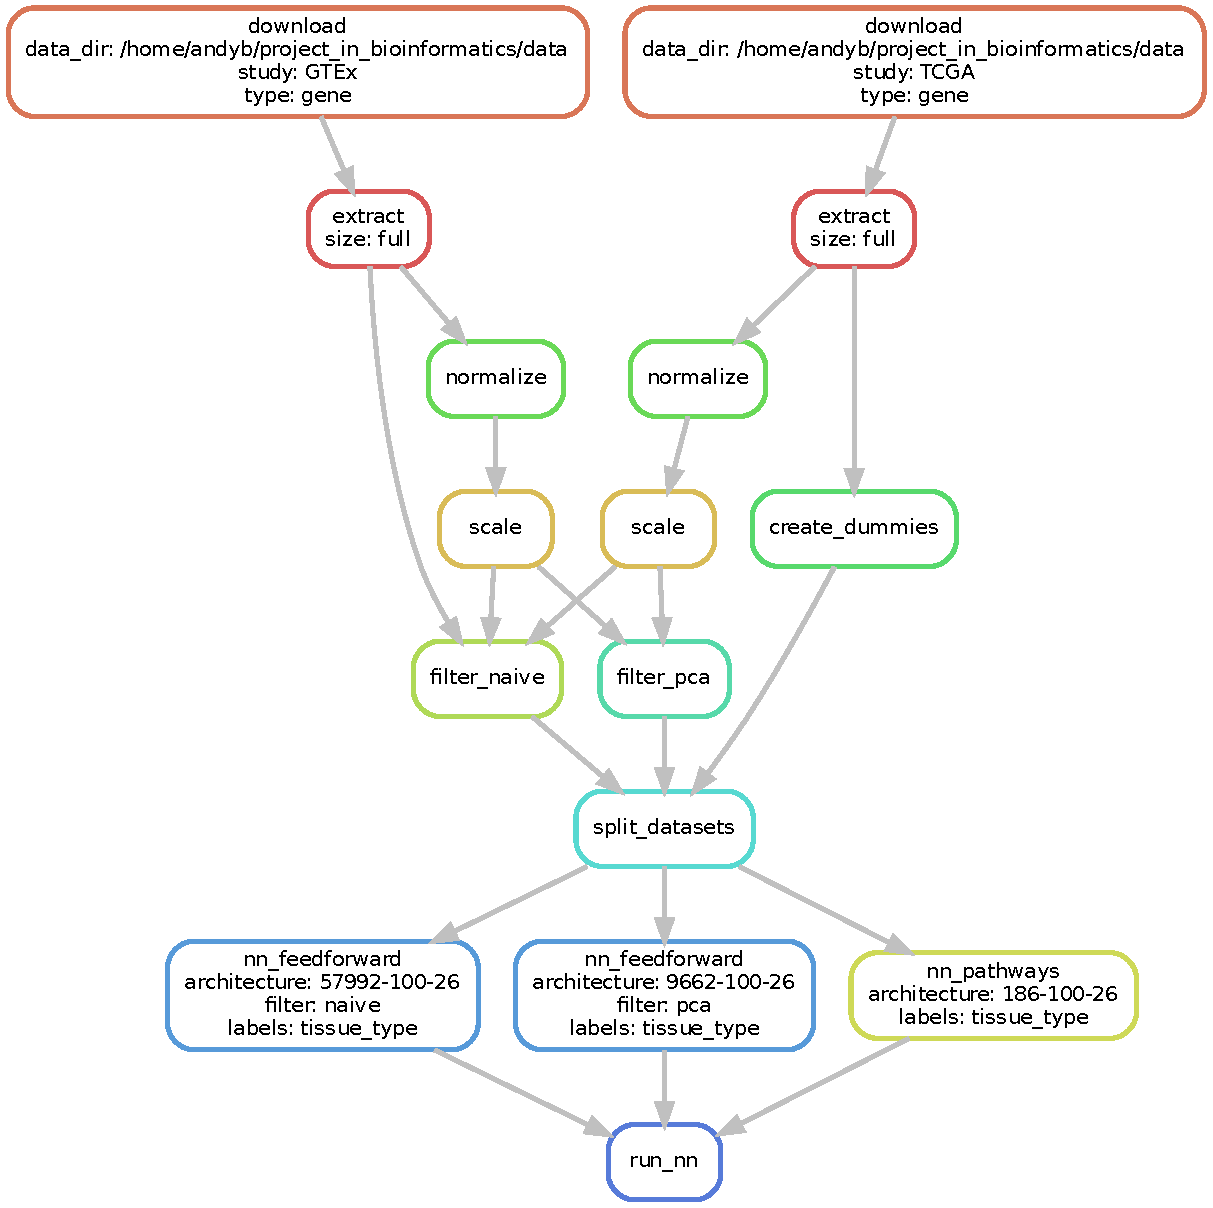
\includegraphics[width=\linewidth]{images/dag.pdf}
    \caption{Pipeline overview: Nodes represent the executed rules, arrows represent the flow of information. This example used fewer parameters in comparison with the real run.}
    \label{fig:dag}
\end{figure}

\newpage
\section{Data available}
The main data which we worked with consisted of RNA-seq gene counts.
RNA sequencing has become a standard in studying a gene expression mainly due to its ability to detect transcriptional activity even without previously defined gene sequence\cite{nellore2016rail}.
A common use of this method is to determine expression level across the samples and then use this information to identify the patterns associated with the outcome of interest.
In our project, we used expression data from two distinct sources, The Genotype-Tissue Expression project (GTEx)\cite{lonsdale2013genotype} and The Cancer Genome Atlas (TCGA)\cite{tcga}.

\subsection{TCGA}
The Cancer Genome Atlas Program is a joint effort between the National Cancer Institute and the National Human Genome Research Institute.
Since the year 2006, they provide access to one of the most comprehensive datasets of multiple types of cancer.
TCGA generated over 2.5 petabytes of genomic, epigenomic, transcriptomic and proteomic data to improve our abilities to diagnose, treat a prevent cancer.
These data are publicly available to researchers all around the world.

\subsection{GTEx}
The Genotype-Tissue Expression project was established to create a data resource to study genetic variation, the regulation of gene expression and other molecular phenotypes.
The dataset contains expression data from multiple reference tissue types and is freely available online.

\subsection{KEGG pathways}
Another database used in our analysis is the Kyoto Encyclopedia of Genes and Genomes (KEGG) \cite{kanehisa2000kegg}.
This database contains information useful for systematic analysis of gene function and linking genomic information with higher order functional information.
The higher order functional information is characterized as cellular processes, such as metabolism, membrane transport, signal transduction and cell cycle.
In the project, we used the information of the gene membership to particular pathways.
\label{subsec:kegg}

\subsection{Downloading}
Downloading of the expression data was done using R package \verb'recount' \cite{collado2017reproducible}.
We created a custom R script for downloading TCGA expression dataset and GTEx expression dataset.
The downloaded expression data were stored as \verb'RangedSummarizedExperiment' object in the file with the extension \verb'.Rdata'.
This object is designed to select data of interest from the large dataset.
The outline of the object structure can be found in Figure \ref{fig:sre}.
In the case of expression data, the rows contain genes and all information related to them, and the columns contain samples and their related information.
Unfortunately, because we wanted to perform our analysis mainly using python programming language, we needed to convert the downloaded data to another format.
We decided to convert files to tab separated values since this format is widely accepted structuralized data format.
Therefore, for each dataset, we created one file containing gene expression counts, mirroring the structure of assays part of the \verb'RangedSummarizedExperiment' object and two files containing assignments of our response variables to the sample ids.

\begin{figure}
    \centering
    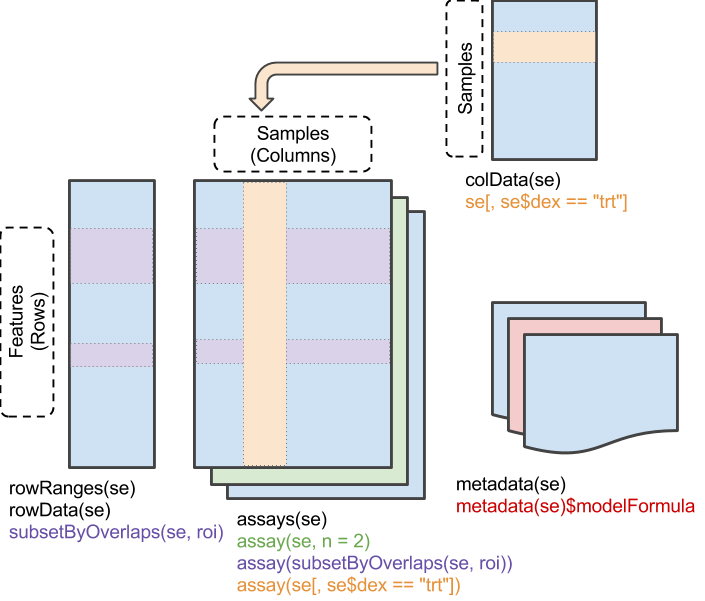
\includegraphics[width=0.8\linewidth]{images/SummarizedExperiment.png}
    \caption{Structure of the RangedSummarizedExperiment object. The rows represent genes, and the columns represent samples. The expression data are stored in the assays part of the object. The structure ensures the correct selection of elements by bounding features to rows and samples to columns.}
    \label{fig:sre}
\end{figure}

\newpage
\section{Data preparation}
Downloaded expression data represented raw counts of the genes.
These raw counts can have multiple problems \cite{robinson2010scaling}.
\begin{enumerate}
    \item Every sample is potentially sequenced to a different depth.
    \item The genes compete for the limited space in the sequencing experiment. Therefore samples with more active genes tend to have lesser expression per gene. 
    \item Genes with longer transcripts have a higher probability of being sequenced.
\end{enumerate}
To mitigate these problems and to ensure high-quality results further down in the pipeline, we performed normalization and scaling of the data.
We also visualized the effects of our normalization and scaling to assess the correctness of our steps.

\subsection{Normalisation}
Because of the different depth in the sequencing experiments, it was necessary to perform normalisation of our data.
The first idea was to divide each expression entry by the median of that particular sample.
This procedure should eliminate the problem with variable depth and potentially the problem with genes competing for limited space in the experiment.  
Unfortunately, in cases with shallow coverage, the median value of the expression was zero, which caused division by zero error in insufficiently covered samples.
Therefore we decided to divide entries by the 75th percentile of a particular sample.
This division had a similar effect as dividing by median, and we overcome the division by zero problems in all samples.
After normalisation with 75th percentile, we also performed a logarithmic transformation of our data.
This procedure helped to reduce the strong left skew of the data and ensured that our data looked more normally distributed.
The effect of this step was visualized in the Figures \ref{fig:expr_dist} and \ref{fig:norm_expr_dist}.

\begin{figure}
    \centering
    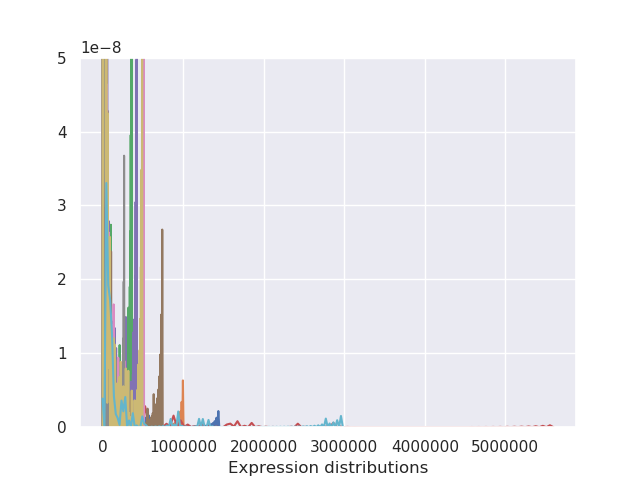
\includegraphics[width=0.8\linewidth]{images/expr_dist.png}
    \caption{Expression distributions of the first 10 samples before the normalization}
    \label{fig:expr_dist}
\end{figure}

\begin{figure}
    \centering
    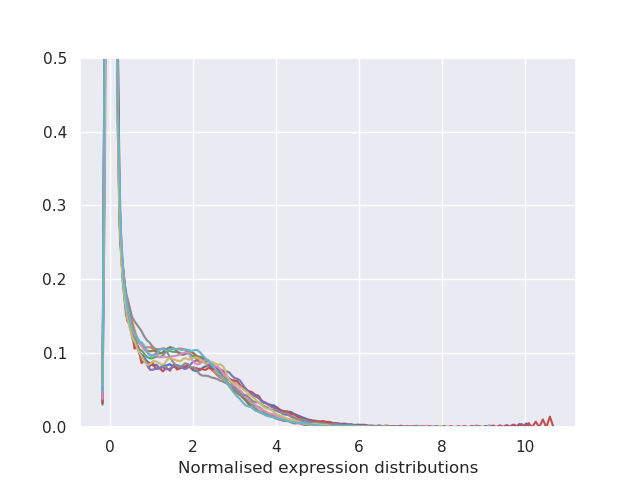
\includegraphics[width=0.8\linewidth]{images/norm_expr_dist.png}
    \caption{Expression distributions of the first 10 samples after the normalization}
    \label{fig:norm_expr_dist}
\end{figure}

\subsection{Scaling}
In the scaling step, we tackled the problem, that longer transcripts tend to have a higher probability of being sequenced.
We decided to solve this issue by adjusting each gene to have mean zero and standard deviation one.
In comparison with the previous step, we performed row-wise standardization instead of column-wise.
Performed standardization was according to the Equation \ref{eq:std}.
The effect of this step was visualized in the Figure \ref{fig:norm_expr_genes} and \ref{fig:scaled_expr_genes}.

\begin{equation}
    x_{ij} = \frac{x_{ij}-\bar{x_{i}}}{sd(x_{i})}
    \label{eq:std}
\end{equation}

\begin{figure}
    \centering
    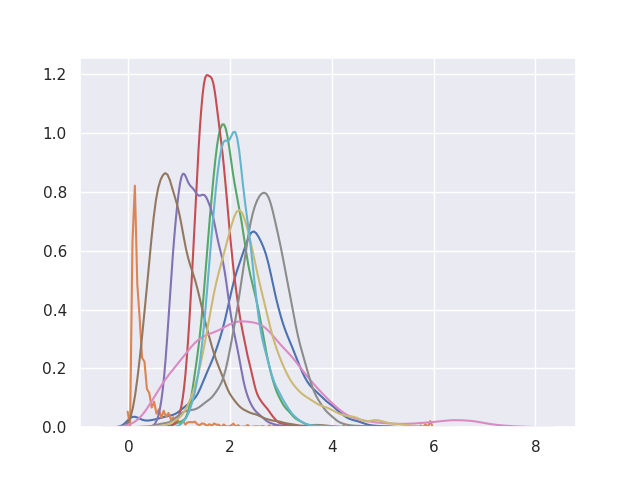
\includegraphics[width=0.8\linewidth]{images/norm_expr_genes.png}
    \caption[]{Expression distribution of the first 10 genes before the scaling}
    \label{fig:norm_expr_genes}
\end{figure}

\begin{figure}
    \centering
    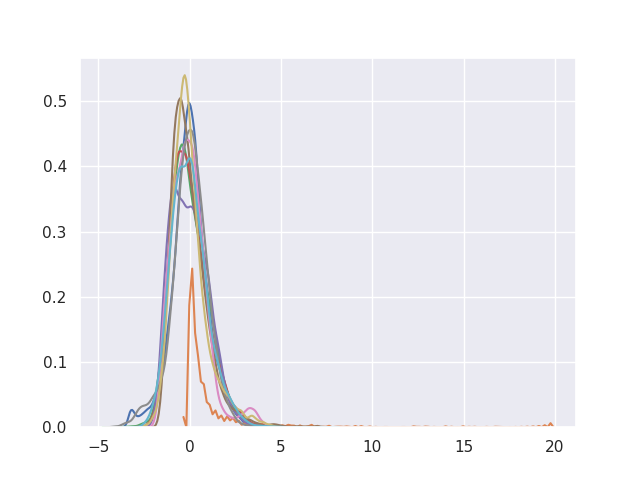
\includegraphics[width=0.8\linewidth]{images/scaled_expr_genes.png}
    \caption{Expression distibution of the first 10 gene after the scaling}
    \label{fig:scaled_expr_genes}
\end{figure}

\newpage
\section{Filtering}
In the filtering step, we tried to select the best predictors for our outcomes.
This step should help the analysis for multiple reasons.
\begin{enumerate}
    \item The number of genes largely exceeds the number of samples. This fact could lead to overfitting and inability to find the model that is general enough to perform well in practice.
    \item There is a considerable probability that some genes are expressed independently of our response variables. We want to remove those genes from the analysis as they introduce noise to our model.
    \item Some gene expressions might be highly correlated. This fact introduces further complications for our model.
\end{enumerate}
To address these issues, we performed feature selection using two different approaches.

\subsection{The variation of within-group means}
The first criterium for good predictor was the variation of within-group means.
The idea was that most non-informative genes tend to have similar values of gene expression in all tissue types.
For this step, we used the GTEx dataset.
We grouped the GTEx data according to their associated tissue type and calculated the mean for each gene in each group.
Afterwards, we calculated the variation of the means for each gene.
The genes in TCGA dataset were then sorted according to the calculated variation in descending order.
The sorted order was then used further in the pipeline, where we chose the first few predictors with the highest variation.

\subsection{Principal component analysis}
Principal component analysis (PCA) is a standard method of dimension reduction for high-dimensional data. 
For $(n\times p)$ matrix, it produces $min(n-1, p)$ principal components.
The principal components are a new set of predictors constructed from the original data in such a way that they are linearly uncorrelated.
In addition, the first principal component explains the most of the variance of the original dataset and each next principal component explains most of the remaining variance under the condition that it is orthogonal to all the previous principal components. 

In our project, we used the GTEx dataset to find the transformation needed to create principal components and then used this transformation on the TCGA dataset.
This transformed dataset was then used further in the pipeline.

\newpage
%
\section{Splitting to training, validation and testing datasets}
Because of the computational intensity of training of the neural networks we decided to validate using validation set. 
This approach can have multiple drawbacks.
% list drawbacks
To mitigate these drawbacks, we decided to perform splitting as follows.
First we removed all observations with missing value of response variable.
These would not help us to train the model.
Then we grouped remaining observations by tissue type and by cancer stage.
From each group we selected 60\% as training set, 20\% as validation set and 20\% as testing set.

\begin{figure}
    \centering
    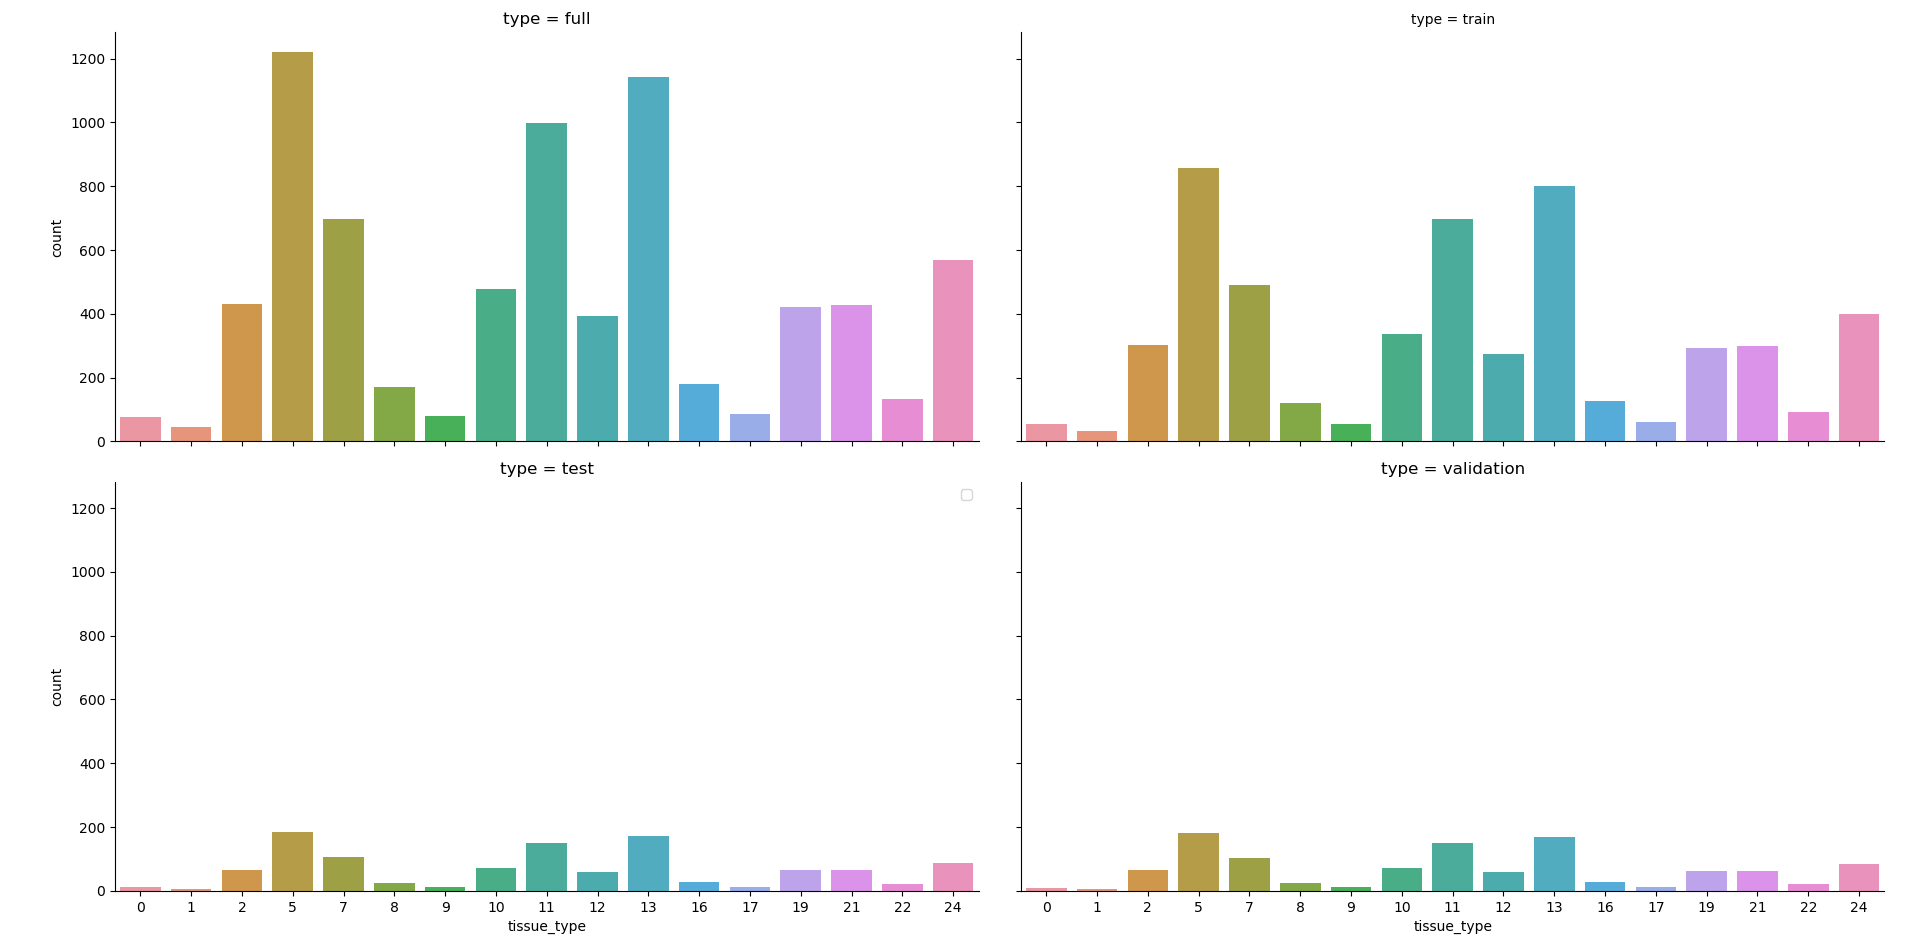
\includegraphics[width=\linewidth]{images/split_tissue.png}
    \caption{Caption}
    \label{fig:split_tissue}
\end{figure}

\begin{figure}
    \centering
    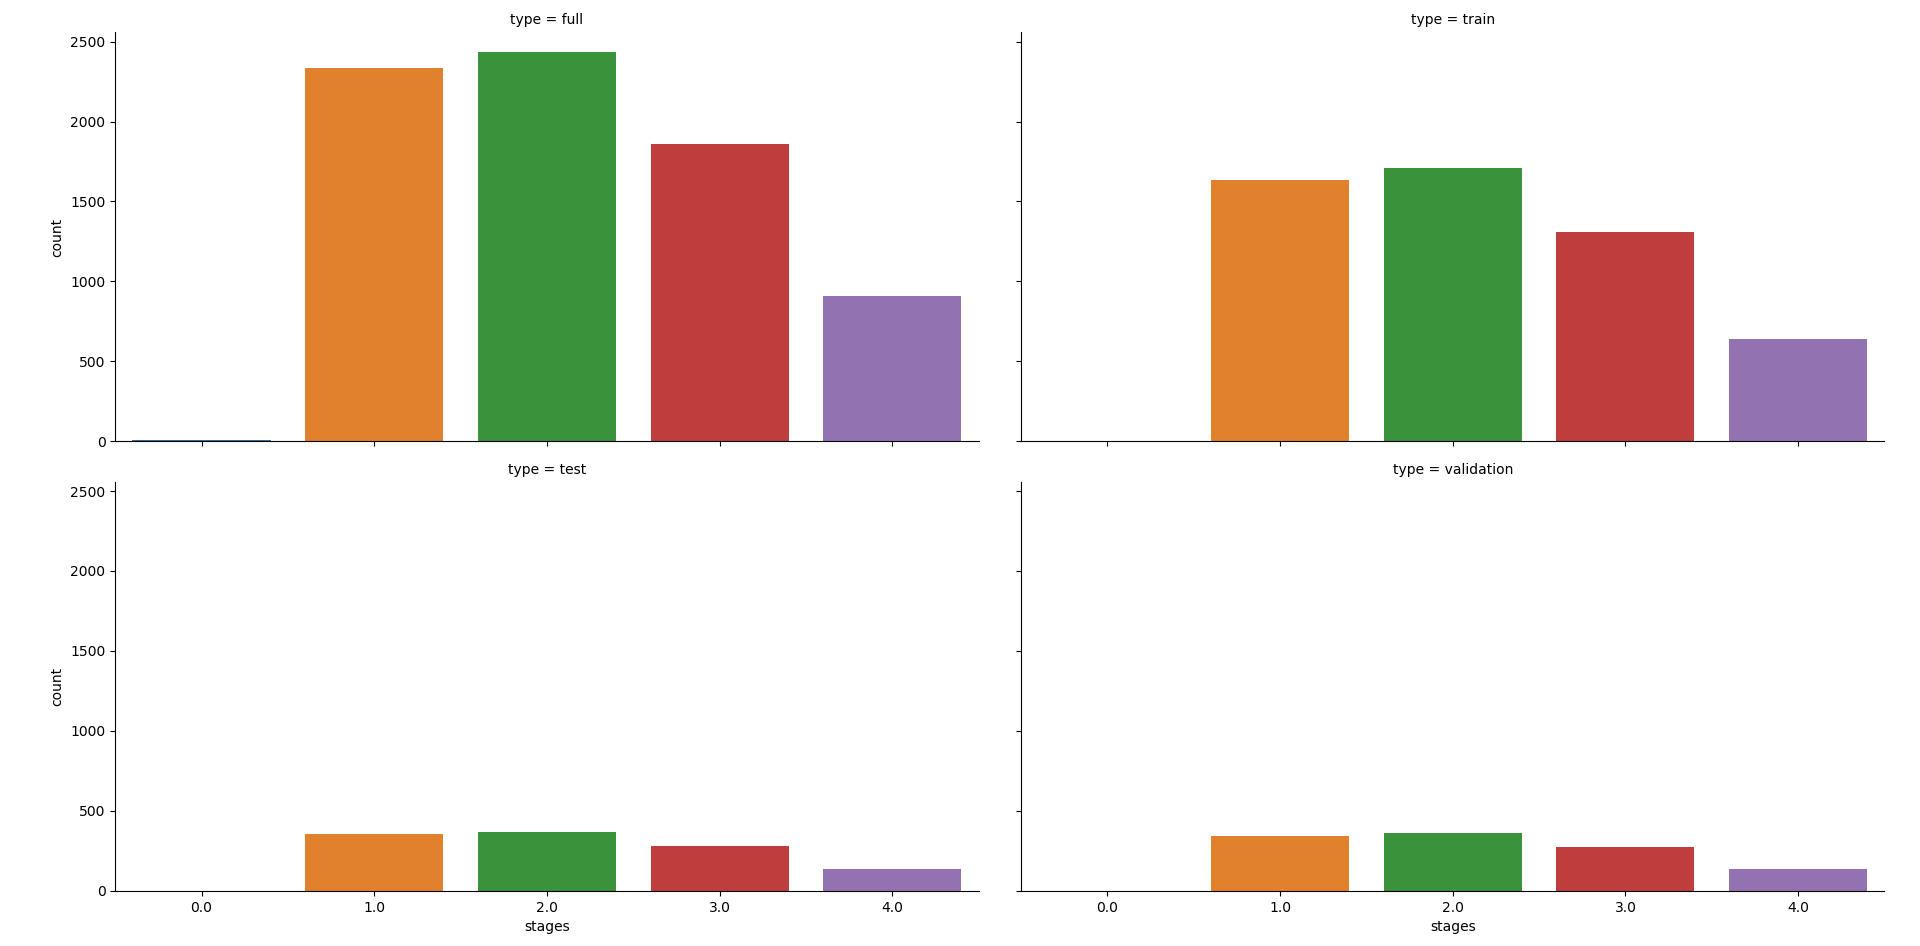
\includegraphics[width=\linewidth]{images/split_stages.png}   
    \caption{Caption}
    \label{fig:split_stages}
\end{figure}

\begin{figure}
    \centering
    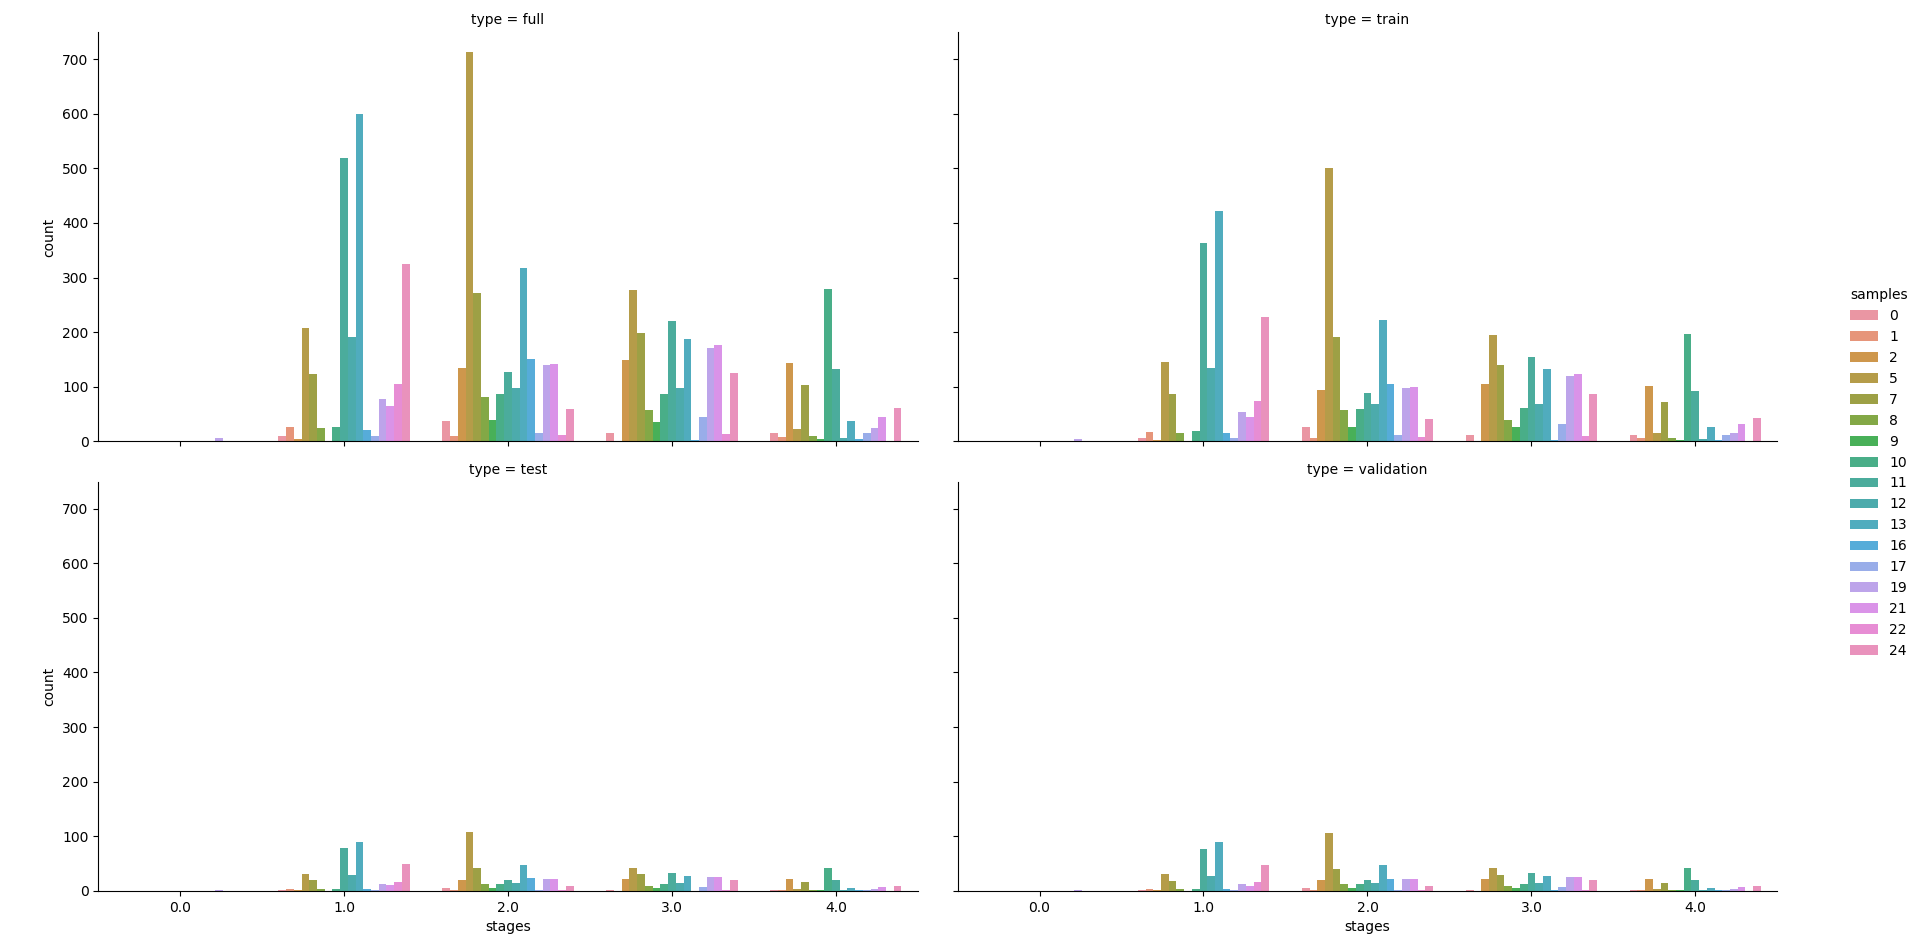
\includegraphics[width=\linewidth]{images/split_all.png}
    \caption{Caption}
    \label{fig:split_all}
\end{figure}

\section{Neural networks}
The main point of this work was to build a neural network classifier for cancer expression data.
Here we will present architecture of neural networks used.

\subsection{PyTorch library}
For building neural networks in this project we used python library PyTorch.
PyTorch library is primarily developed by Facebook's artificial inteligence research group. \cite{pytorch}
In comparison with other AI frameworks, PyTorch belongs to one of the most popular with wide support for scientific community.
It is a lower-level API directly focused on work with array expression which directly encourage the understanding of deep learning concepts.
Its lower-level approach also ensures, that the programmer has more control over the architecture.
Despite its lower-level approach it still provides automatic differentiation and backpropagation.

\subsection{Dataset object}
PyTorch provides an option to define custom dataset.
This is preferable way to use data when training the neural network, because it makes the code more clean and intuitive.
It also enables to train the model on batches which can be even shuffled.
This can make the process of training more stable and less likely to jump over some good values of parameters.
In our project we made use of these benefits of using abstract Dataset class and created custom class MyDataset extending the Dataset class.

\subsection{Feed forward neural network}
Next step was to define neural network.
We made our neural network class parametrized by the parameter architecture.
This parameter was in the format INT-...-INT, where first integer represented the size of input layer of desired neural network, last integer represented the size of output layer and all integers in the middle represented the sizes of hidden layers.
This was done using PyTorch object ModuleList to which we then added Linear layers with required parameters.
For each hidden layer we used ReLU as nonlinearity function.

\begin{figure}
    \centering
    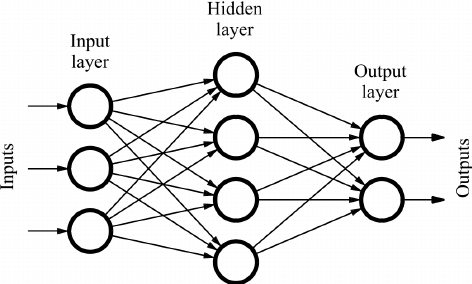
\includegraphics[width=0.8\linewidth]{images/ff_nn.png}
    \caption{Typical neural network architecture.}
    \label{fig:ff_nn}
\end{figure}

\subsection{Pathways neural network}
In this architecture we wanted to incorporate additional information about the genes into the neural network.
For this we used KEGG data mentioned in Subsection \ref{subsec:kegg}.
First layer in the pathways neural network was our custom layer Pathways.
This layer represented membership of a gene to a particular biochemical pathway.
This was done using the binary matrix where rows represented genes and columns represented pathways.
Our custom layer then performed entrywise matrix multiplication between binary matrix and weights.
This effectively set majority of the connections to zero and the remaining connections were the one representing membership of the gene to a pathway.
This new matrix was then used for transition between input layer to the first hidden layer.
From the first hidden layer to the output layer we used Linear layers similarly to the Feed forward neural network.

\subsection{Training and regularization of the neural networks}
During the training we loaded training observations to out custom dataset class.
This class was then passed to the built in DataLoader class which allowed us to train in shuffled batches.
We also programmed this training procedure to be able to use graphical processing unit (GPU) for better performance.
As an optimized we used Adam - adaptive moment estimation \cite{kingma2014adam} optimizer with BCEWithLogitsLoss loss function. 
After each run through the whole training dataset we recorded the training loss, training accuracy, validation loss and validation accuracy.
We also stored a pickled python object of the model after each epoch.
The idea here was to perform a form of regularization, where we would choose the model with lowest validation error.
Together with this regularization, we also used dropout regularization.
Furthermore, we also tried L2 regularization. 
To estimate the hyperparameter which should be used by L2 regularization, we ran through multiple options.
The validation error using the L2 regularization can be found in the Figure \ref{fig:L2_reg}.

\begin{figure}
    \centering
    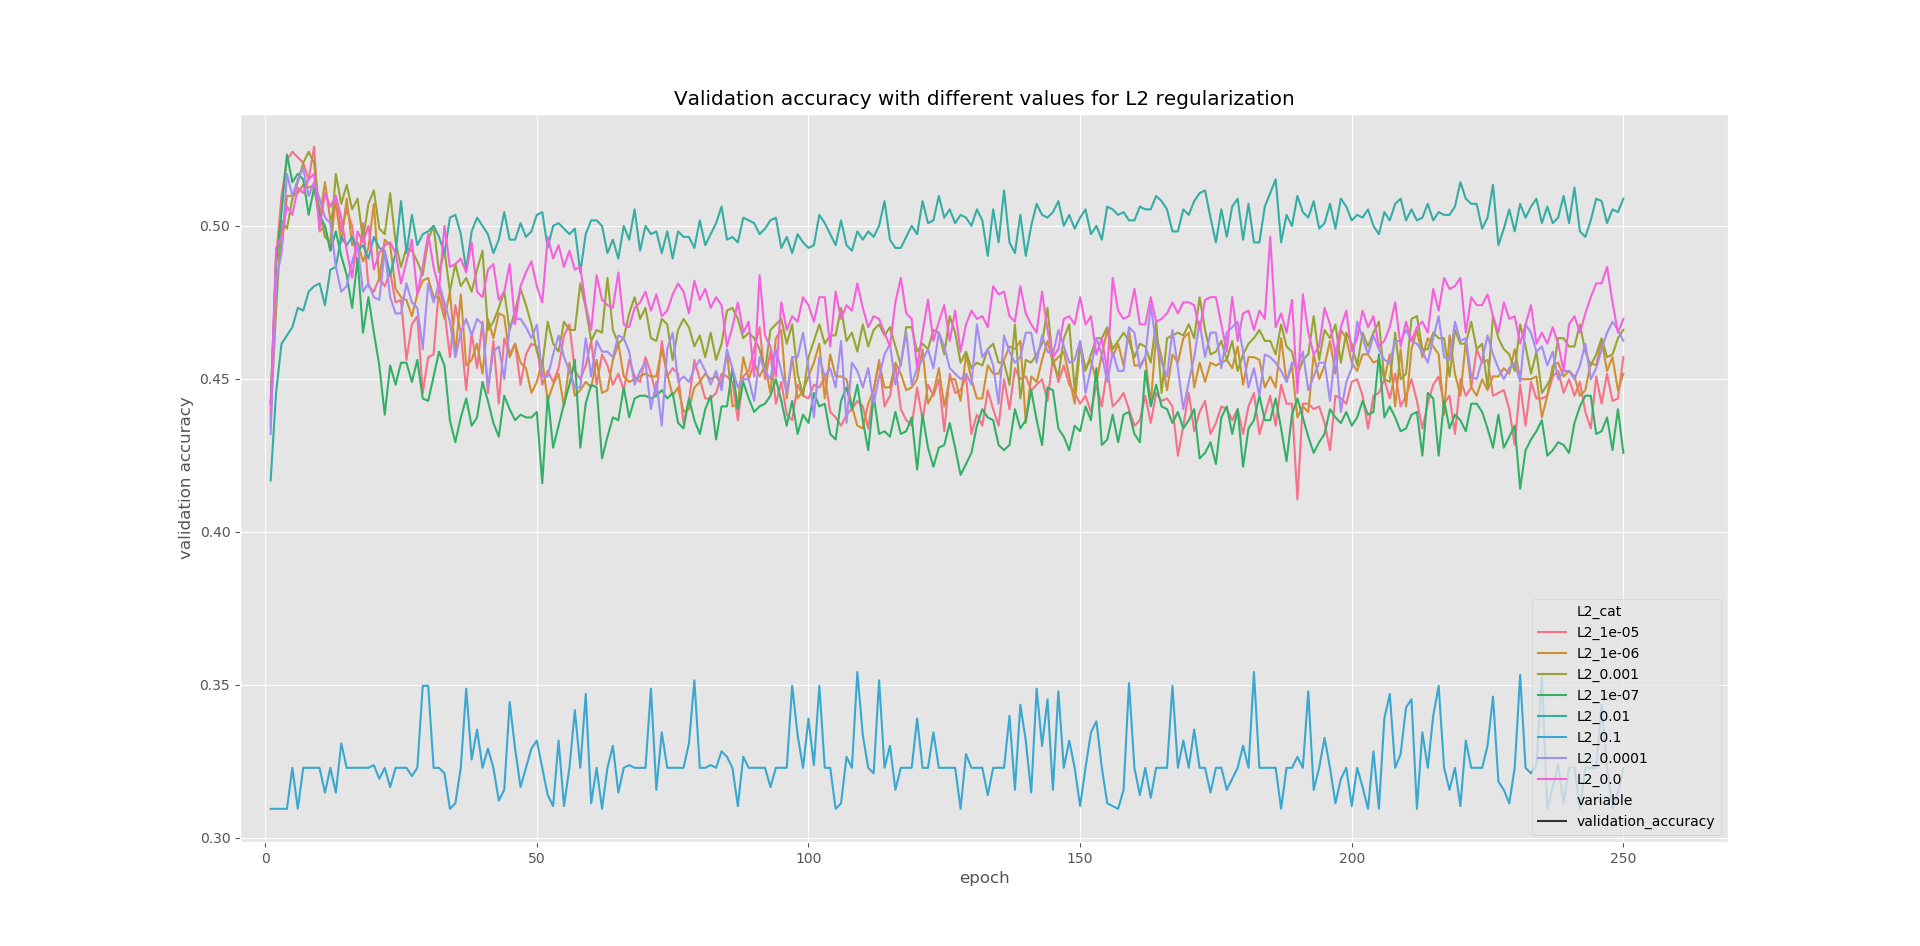
\includegraphics[width=\linewidth]{images/val_acc_l2.png}
    \caption{}
    \label{fig:L2_reg}
\end{figure}

Unfortunatelly, L2 regularization did not improve our accuracy over the model with just dropout, therefore we decided not to use it.
